\chapter{Theory of (Mis)communication}
\label{chap:theory}

In the previous chapter, I discussed findings from a study that explored reasons developers have for not using program analysis tools. One reason that almost all developers in that student could agree on is that the output provided by their tools are sometimes difficult to interpret.
Therefore, this chapter presents research that took a deep dive to explore the challenges developers encounter when interpreting tool notifications.

To answer the question \emph{why do developers encounter challenges when interpreting program analysis tool notifications?}, I observed 26 developers with varying backgrounds while they used three different program analysis tools: Eclipse Java compiler, FindBugs, and EclEmma. I presented participants with and asked them to interpret notifications from each of the three tools. 
To identify challenges, I examined tool use through the lens of communication theory~\cite{bowman1987modeling}.
Building on an existing model of (mis)communication~\cite{mustajoki2008modelling}, I identified 12 kinds of challenges developers encounter when interpreting tool notifications.

% TODO should this come first or after challenges listed?
Based on the challenges participants encountered when interpreting tool notifications, I proposed a tool miscommunication theory that can be used to inform the design of program analysis tools.
Experts in qualitative research suggest that rather than presenting a set of disparate findings, qualitative researchers should instead produce an explanatory theory, a ``skeleton or framework that explains why things happen''~\cite{corbin2014basics}. While explicitly putting forward theories is rare in software engineering~\cite{hannay2007systematic}, one example is Lawrance and colleagues' theory of how programmers navigate code during debugging~\cite{lawrance2013programmers}. In the same way that Lawrance and colleagues' build on 
information foraging theory~\cite{pirolli1999information}, my theory builds on communication theory~\cite{bowman1987modeling}.
I summarize my theory as:

\begin{quotation}
	\noindent
	\emph{The challenges developers encounter when interpreting program analysis tool notifications are caused by gaps and mismatches between developer knowledge and how notifications communicate information.}
\end{quotation}

In the following sections, I will discuss the methodology I used to identify developer challenges, the 12 kinds of challenges I identified that informed this theory, and ways in which this theory can be operationalized.

\section{Identifying Challenges}

% TODO this probably becomes an Appendix reference (or maybe separate ones for each thing that can be referenced)
% Research materials are available on-line to aid other researchers in replication and exploration.\footnote{\url{http://www4.ncsu.edu/~bijohnso/esnpat.html}}

%\subsection{Research Question}\label{rq}

In a previous study, I asked developers to recall experiences with static analysis tools and briefly use FindBugs. I found that some developers do not use program analysis tools due to difficulty interpreting the notifications tools use to communicate~\cite{johnson2013don}. 
To find out how tools could better communicate with developers, this study was designed to answer the
question: \noindent\emph{Why do developers encounter challenges when interpreting program analysis tool notifications?} Using Hannay and colleagues' guidelines~\cite{hannay2007systematic}, 
I framed my question as \emph{why} rather than \emph{what} to support the building of a theory that explains the challenges developers encounter.

\begin{figure*} [ht]
\centering
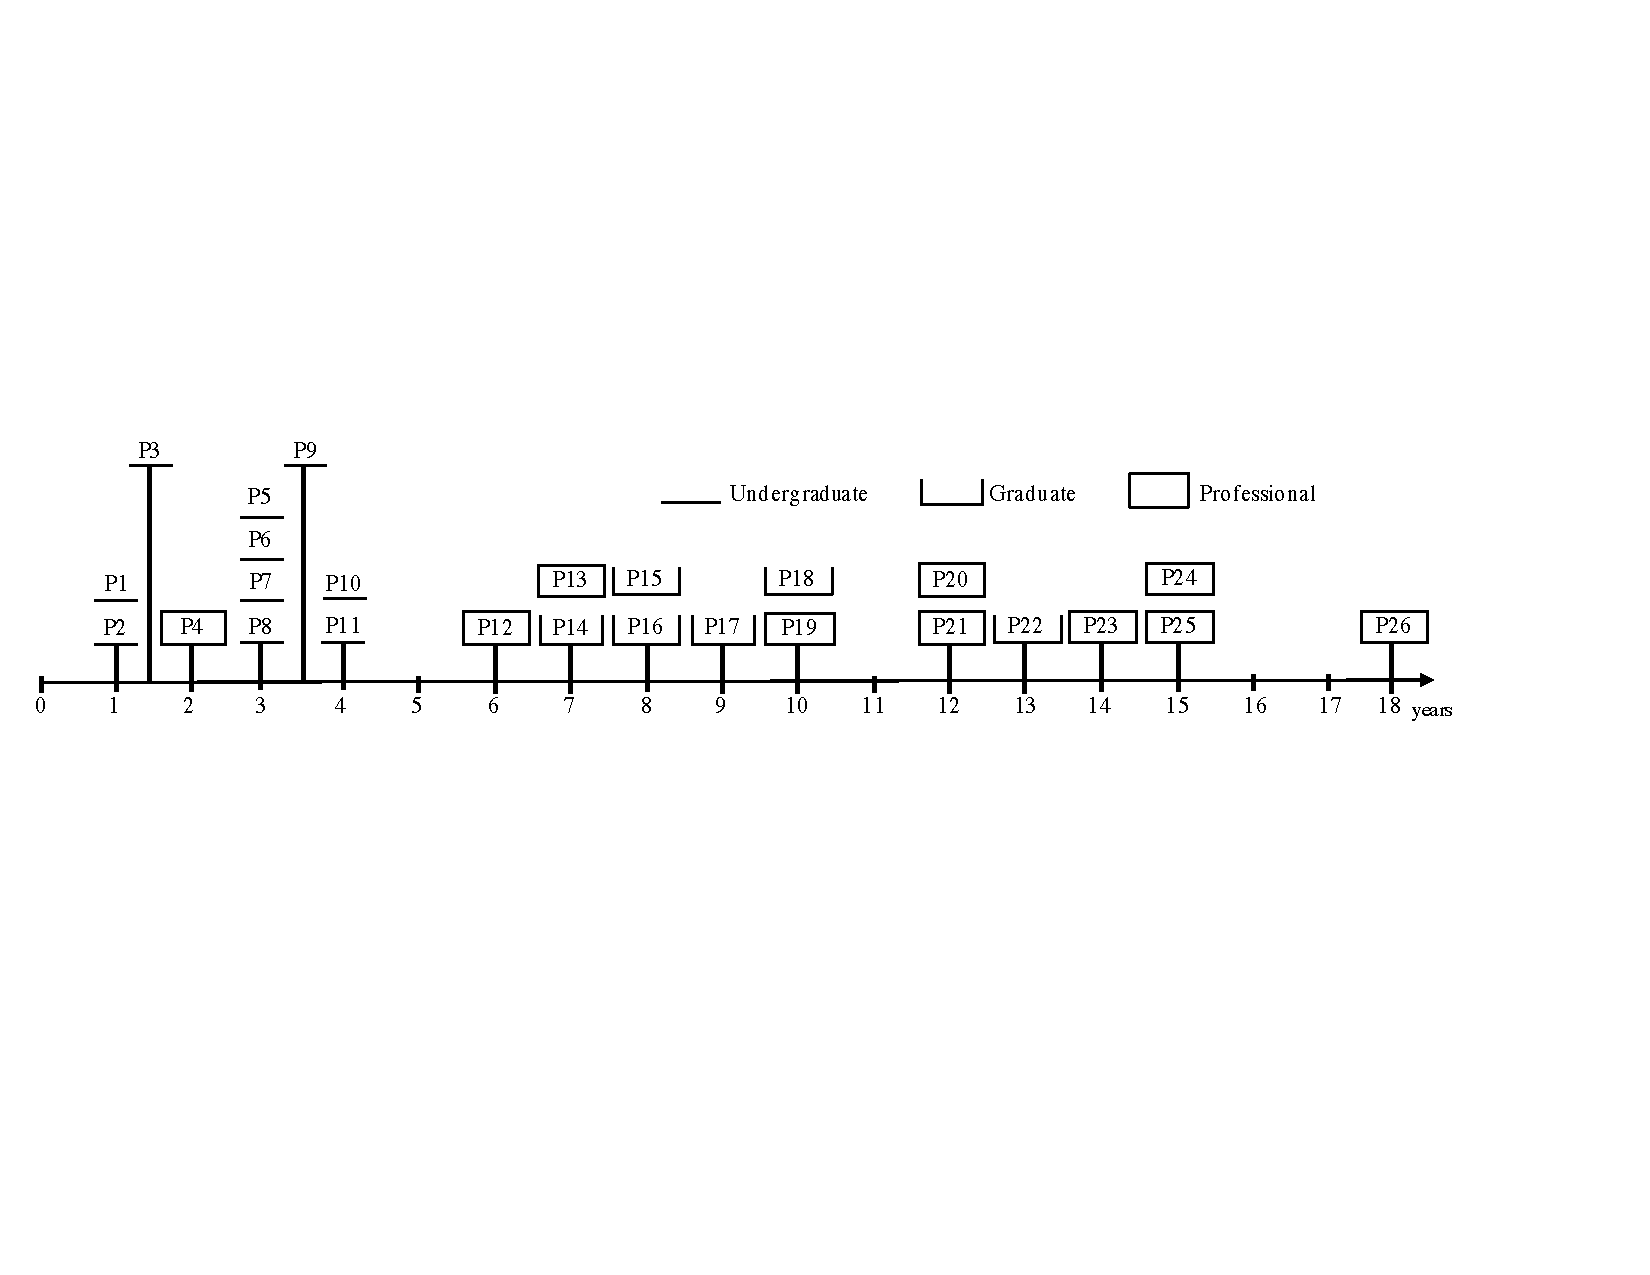
\includegraphics[width=\textwidth]{Chapter-4/figs/participants.pdf}
\caption{Distribution of participants based on years of programming
experience.}
\label{fig:participants}
\end{figure*}

\subsection{Participants} \label{participants}

I recruited twenty-six participants using mailing lists, classroom recruitment, and personal
contacts. Participants included undergraduate students, graduate students, and
professional developers, with varying amounts of development and tool
usage experience. Figure~\ref{fig:participants} shows the distribution of
participants' development experience, based on self-reports in a pre-study
questionnaire. 
Increasing participant numbers indicate increasing software development experience,
and throughout this chapter, I use \professional{boxes} or \graduate{partial} 
\undergraduate{boxes} to indicate participant job roles (professional, graduate, and undergraduate respectively).
For example, the figure indicates that \professional{P24} is a professional developer with fifteen years of development experience. 
Three graduate students (\graduate{P15}, \graduate{P18}, \graduate{P22}) reported having industry experience.
Ten participants had prior experience using EclEmma. 
Nineteen participants had prior experience with FindBugs. 
All participants had experience with the Eclipse Java compiler.

\subsection{Program Analysis Tools Investigated} \label{TUI}

This study focused on tools that can be used in the Eclipse
Integrated Development Environment (IDE)~\cite{EclipseIDE}. 
I chose Eclipse because it is one of the most widely used IDEs~\cite{Goth:2005:Beware}, 
making it easier to recruit qualified participants,
and because it is compatible with a variety of tools. I selected FindBugs, the Eclipse Java Compiler, and
EclEmma as mature, popular tools.


\subsubsection*{FindBugs}

FindBugs (version 2.0) notifications communicate with the developer about defects in her
code based on code patterns. Bug icons (
\includegraphics[height=9px]{Chapter-4/figs/bug}) in the gutter are colored red
to indicate the ``scariest'' code patterns, orange for ``scary'' patterns, yellow
for ``troubling'' patterns, and blue for ``of concern.'' Text descriptions are
available by hovering over or clicking the 
\includegraphics[height=9px]{Chapter-4/figs/bug} icon as seen in Figure~\ref{fig:N4}.

\begin{figure} [t]
	
	\subfigcapskip = 1pt
	\subfigure[Source Code]{
		\fcolorbox{lightgray}{white}{\parbox{\dimexpr\linewidth-5\fboxsep-2\fboxrule}{
				\centering 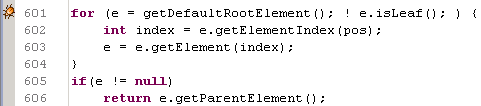
\includegraphics[width =3.3in] {Chapter-4/figs/N4(no_tooltip)}
			}}
			
		}
		
		%The space between the figure and the caption
		\subfigcapskip = 1pt
		\subfigure[Short Description]{
			%From http://tex.stackexchange.com/questions/120530/wrapping-text-inside-framebox
			%\framebox (or fcolorbox) makes the box around the text.  The \parbox allows for wrapping
			%The \dimexpr stuff makes it fit in the column.  You don't need manual
			\fcolorbox{lightgray}{white}{\parbox{\dimexpr\linewidth-2\fboxsep-2\fboxrule}{
					{\centering \scalebox{.8}{Nullcheck of e at line 605 of value previously dereferenced in \texttt{javax.swing.text.DefaultStyledDocument.}}\\
						\scalebox{.8}{\texttt{getParagraphElement(int)} } \\
					}
					
					
				}}
				
			}
			\subfigcapskip = 1pt
			\subfigure[Full Description]{
				\fcolorbox{lightgray}{white}{\parbox{\dimexpr\linewidth-2\fboxsep-2\fboxrule}{
						
						{\centering \scalebox{.8}{A value is checked here to see whether it is null, but this value can't be null because it was previously dereferenced} \\
							\scalebox{.8}{ and if it were null a null pointer exception would have occurred at the earlier dereference. Essentially, this code and} \\ 
							\scalebox{.8}{  the previous dereference disagree as to whether this value is allowed to be null. Either the check is redundant } \\ 
							\scalebox{.8}{or the previous dereference is erroneous.} \\ 

						}
						
						
					}}
				}
				\caption{A notification of a previous null check from FindBugs (FB4).}
				\label{fig:N4}
			\end{figure}

\subsubsection*{Eclipse Java Compiler}

Eclipse Java compiler (JDT version 3.8) notifications communicate with developers when their program cannot
compile and provide warnings about suspicious code~\cite{EclipseCompiler}.
Notifications are typically shown as squiggly underlines in the editor. Like FindBugs, the compiler uses color to represent severity; errors
are shown as red underlines, warnings as yellow underlines.
Underlines are augmented with gutter icons
(
\includegraphics[height=9px]{Chapter-4/figs/comp-x}), as shown in
Figure~\ref{fig:notificationCOMP} at line 159. When the developer mouses over
the underlined code or the 
\includegraphics[height=9px]{Chapter-4/figs/comp-x} icon, the
notification displays a text description (Figure~\ref{Comptext}). Unlike FindBugs, clicking the gutter icon does not provide a detailed description. Instead, clicking the icon sometimes provides possible fixes that can be automatically applied to the code called quick fixes.

\begin{figure} 
\subfigcapskip = 1pt
\centering
\subfigure[Source Code]{
   \fcolorbox{lightgray}{white}{\parbox{\dimexpr\linewidth-2\fboxsep-2\fboxrule}{
	 \centering 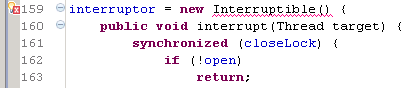
\includegraphics[width=3.3in]{Chapter-4/figs/comp-notification}
	
}}}
\subfigcapskip = 1pt
\subfigure[Text Description]{
\fcolorbox{lightgray}{white}{\parbox{\dimexpr\linewidth-2\fboxsep-2\fboxrule}{
	
{\centering \scalebox{.8}{The type \texttt{new AbstractInterrruptibleChannelInterruptible()} must implement the inherited abstract  } \\
  \scalebox{.8}{\texttt{method new AbstractInterruptibleChannel.Interruptible.interrupt()}}
}


}} }

\caption{An Eclipse compiler notification about unimplemented methods (CMP5).}
\label{fig:notificationCOMP} 
\end{figure}

\subsubsection*{EclEmma}

EclEmma (v2.2) is a code coverage tool that executes a program, typically with JUnit
as the driver~\cite{JUnit}, to communicate with the developer about code paths that did and
did not get exercised. Although EclEmma communicates about one particular execution, 
as with the other tools it provides information to the developer regarding code 
(during runtime rather than compile-time). 
EclEmma uses highlighting to indicate code execution; code highlighted in
green was executed, red was not executed, and yellow was partially executed.
Figure~\ref{fig:notificationECL} shows an example of coverage reported by
EclEmma on an \texttt{if} statement. When the developer mouses over the

\includegraphics[height=9px]{Chapter-4/figs/diamond} icon, the tool notifies her of how many
paths got executed on the associated branch statement at line 133
(Figure~\ref{Ecltext}).

\begin{figure} [t]
\subfigcapskip = 1pt
\centering
\subfigure [Source Code with Highlighting]{ 
\fcolorbox{lightgray}{white}{\parbox{\dimexpr\linewidth-2\fboxsep-2\fboxrule}{
    \centering 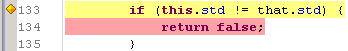
\includegraphics[width=3.3in]{Chapter-4/figs/EclExample}
	
}}}
\subfigcapskip = 1pt
\subfigure[Text Description]{
\fcolorbox{lightgray}{white}{\parbox{\dimexpr\linewidth-2\fboxsep-2\fboxrule}{
	\centering
	{\small ~~~1 of 2 branches missed~~~ }
   
}}
}

\caption{An EclEmma notification about partial branch coverage (ECL3).}
\label{fig:notificationECL}
\end{figure} 

These tools may seem quite different, but I chose them
specifically to identify challenges developers experience \emph{across} tools.
Despite the differences, these tools attempt to communicate similar concepts to developers using similar textual and visual notifications.
For example, both FindBugs and EclEmma communicate information about 
control flow, and both FindBugs and the Eclipse Java Compiler communicate about data flow.
All three tools use color codes in a largely consistent manner, 
such as using red to indicate the highest level of urgency.
And as a final example, most notifications communicate information about program elements, such as methods and classes, and information about program execution, be it potential or actual.


\begin{table*} 
\rowcolors{2}{white}{gray!25}
\centering
\caption{Notifications used in our study}
\begin{tabular}{llll}
%\rowcolor{gray!50}
	\hline
    \textbf{Notification} & \textbf{Tool} & \textbf{Problem} & \textbf{Category} \\
	\hline

%tildes just padding out to \textwidth
    FB1~~~~~~~~~~~~~~~~~& FindBugs~~~~~~~~~~~~~~& \begin{tabular}[c]{@{}l@{}}String comparison \\using == or !=\end{tabular}~~~~~~~~~~~~& Pointers/References\\
    FB2			    & FindBugs      	  		& \begin{tabular}[c]{@{}l@{}}Incorrect Lazy \\ Initialization\end{tabular} 		    			& Multi-threading		\\
    FB3 				& FindBugs     		  		& \begin{tabular}[c]{@{}l@{}}Synchronize on \\ mutable field\end{tabular}						& Multi-threading	    	\\
    FB4				& FindBugs     		  		& \begin{tabular}[c]{@{}l@{}}Redundant null check\end{tabular} 									& Null/Pointers/References	     	\\
    FB5				& FindBugs       	  		& \begin{tabular}[c]{@{}l@{}}Possible null \\pointer dereference\end{tabular}						& Null/Pointers/References		\\
    CMP1				& Eclipse Compiler    & \begin{tabular}[c]{@{}l@{}}Unused code\end{tabular}							    				& Dead Code	\\
    CMP2				& Eclipse Compiler    & \begin{tabular}[c]{@{}l@{}}Unchecked Conversion, \\Raw Type\end{tabular}							& Generics              \\
    CMP3				& Eclipse Compiler    & \begin{tabular}[c]{@{}l@{}}Unimplemented methods\end{tabular}									& Inheritance/Polymorphism	  		 \\
    CMP4			    & Eclipse Compiler    & \begin{tabular}[c]{@{}l@{}}Serializable class \\needs serial ID\end{tabular}						& Serialization	              \\
    CMP5			    & Eclipse Compiler    & \begin{tabular}[c]{@{}l@{}}Unimplemented methods\end{tabular} 									& Inheritance/Polymorphism	          		\\
    CMP6    			& Eclipse Compiler    & \begin{tabular}[c]{@{}l@{}}Method not applicable \\for arguments\end{tabular}						& Inheritance/Polymorphism	            \\
    ECL1				& EclEmma		      		& \begin{tabular}[c]{@{}l@{}}Red class with \\red class header\end{tabular} 					& Class/test coverage	        	\\
    ECL2				& EclEmma       	  		& \begin{tabular}[c]{@{}l@{}}Red class \\(constructor only)\end{tabular}						& Class/test coverage	            	\\
    ECL3				& EclEmma       	  		& \begin{tabular}[c]{@{}l@{}}Simple if statement\end{tabular}								& Branch/test coverage	   		\\
    ECL4				& EclEmma       	 		& \begin{tabular}[c]{@{}l@{}}Return statement \\with branches\end{tabular}					& Branch/test coverage                \\
    ECL5				& EclEmma			  		& \begin{tabular}[c]{@{}l@{}}Try/Catch/Finally \\(coverage varies)\end{tabular}				& Test coverage, Exception handling	           	 \\
    ECL6				& EclEmma       		 	& \begin{tabular}[c]{@{}l@{}}Nested if statements\end{tabular}								& Branch/test coverage              \\
    \hline
\end{tabular}
\label{table:notifications}
\end{table*}

\subsection{Study Protocol}

Each session with a participant lasted approximately one hour.
Prior to each session, participants filled out a consent form
and pre-questionnaire.\footnote{This work was approved under IRB No. 2787.} 
Each session consisted of seventeen tasks.

Source code for the tasks came from OpenJDK~\cite{OpenJDK} and JFreeChart~\cite{JFreeChart}.
I chose Open JDK because it has a large code base from which I could easily
find bugs using their publicly available FindBugs cloud
report~\cite{FindBugsCloud}. I chose JFreeChart because it is a large code
base with working JUnit test cases that exhibit less-than-perfect code coverage.

For each task, I presented participants with and asked them to interpret one or more notifications from a given tool.
I disallowed the use of a web browser to isolate the challenges developers encounter to the notifications used by the tools and to exclude challenges caused by outside tools or resources.
Allowing use of the browser would have added data that does not help answer the current research question.
I also wanted to see if developers could interpret tool notifications without the aid of outside resources. 
During many tasks, and at least once for every participant, participants
discussed or completed notification resolution. I did not require them to do so as the focus of this study was on the ability to interpret, not to resolve.
As participants explained the notifications, the first author asked follow-up
questions as necessary. 

% EDITED BASED ON REVIEWER COMMENT
Table~\ref{table:notifications} shows a list of the notification tasks participants encountered during each session. A more detailed listing, with screenshots, of the notifications used in this study can be found in Appendix~\ref{chap4:artifacts}. 
For each task, I chose notifications to represent the types of notifications developers may encounter when programming.
For FindBugs and the Eclipse compiler, I chose notifications that appeared frequently in the OpenJDK project. 
I chose EclEmma notifications from JFreeChart to exercise a range of its coverage scenarios. 
Because EclEmma's documentation did not specify the range of notifications it uses, 
I manually went through JFreeChart's codebase after running the tool and took note of 
each new coverage scenario encountered.
I then included an example of every coverage scenario in the EclEmma tasks.

\begin{figure} 
\subfigcapskip = 1pt
\centering
\subfigure[Source Code]{
   \fcolorbox{lightgray}{white}{\parbox{\dimexpr\linewidth-2\fboxsep-2\fboxrule}{
	 \centering 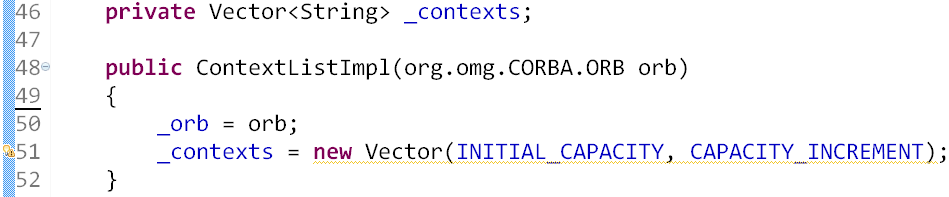
\includegraphics[width=3in]{Chapter-4/figs/CMP2}
	
}}}
\subfigcapskip = 1pt
\subfigure[Text Description]{
\fcolorbox{lightgray}{white}{\parbox{\dimexpr\linewidth-2\fboxsep-2\fboxrule}{
	
{\centering \scalebox{.8}{- Type safety: The expression of type Vector needs unchecked conversion to conform to Vector<String>.}\\
		\scalebox{.8}{- Vector is a raw type. References to generic type Vector<E> should be parameterized.}\\
}


}} }

\caption{A notification from the compiler about generics (CMP2).}
\label{fig:CMP2} 
\end{figure}

For FindBugs, each task during the session corresponded to a single
notification.
All but one compiler task corresponded to a single notification;
because the two notifications on CMP2 (Figure~\ref{fig:CMP2}) contribute to the same problem on the same line, I presented them as one task. 
%TODO explain ``CMP'' notation, as well as participant notation.
Each EclEmma task consisted of participants explaining coverage notifications for the entire class. 

\subsection{Data Collection}

I recorded audio and the screen in each session for analysis.
I then created transcripts from the audio, 
and included descriptions of actions that a participant performed 
that were relevant to interpreting the notification. 
For example, if a participant navigated to different parts of the code 
but did not explicitly describe it, 
I added a description of that navigation to the transcript.

\subsection{Data Analysis}

I analyzed each session using open and selective coding~\cite{corbin2014basics} to discover participant challenges. 
To identify a challenge, I needed concrete criteria. 
I proposed that tool use is a form of communication, and therefore that challenges when interpreting a notification can be seen as ineffective communication.
Existing research on how computers should talk to people suggests that if an explanation is required for a message to be understood, the message was not effective~\cite{dean1982computer}.

I used this logic to determine when a challenge occurred, using three criteria for inclusion: 
\begin{enumerate}
    \item The participant explicitly stated a challenge.
    \item The participant was unable to explain the notification.
    \item The participant had to take steps, outside of reading the notification, to deduce the problem.
\end{enumerate}

Whether an observation met a criterion is independent of whether the participant was able to explain the notification.

I and a collaborator individually used open coding on each transcript, labeling portions that mapped to a challenge. We then reconvened to merge our codes. The criteria above guided this process; if we could not agree that a code fit our criteria, we removed it from our data set. 
Of the 404 codes we originally extracted, we disagreed on 82 (20\%) from twenty-six sessions. 
To resolve our disagreements, we referred to our criteria; if we could not come to an agreement regarding the code fitting the criteria, we removed the statement from our data set. 
For four sessions, we had no disagreement.
In the end, we identified 322 codes. We put each code onto a note card, along with the participant and tool being used. 

Next, I used a card sorting methodology similar to that of Mu\c{s}lu and
colleagues~\cite{Muslu:2014:Transition}. 
The goal of this card sort was to identify themes based on the identified codes.
I used five of the eight authors on the publication of this work and completed the card sort in three phases. In phase 1, we sorted all cards into high-level themes; each card could only go in one theme. s
Phase 2 focused on determining where high-level themes could be broken down into lower-level themes.
In phase 3, we focused on making sure that each card was in the best fitting theme. During this phase, we also clarified theme definitions and made note of example statements to represent each theme.

Because one of the criteria is participant inability to explain a notification, 
any actions or statements made surrounding that occurrence was included in the card sort. 
Upon reflection, some emergent themes took the form of consequences rather than challenges, 
such as notification resolution without understanding and lack of trust in the tool, 
therefore I will not discuss them in this chapter. 
I likewise will not discuss the emergent theme of tool feature requests.
% TODO isthis another appendix??
These excluded themes are available with the other on-line research materials.

\subsection{Study Credibility \& Findings Validation}

There are inherent threats to the validity of empirical 
research~\cite{onwuegbuzie2007validity}.
Despite these inherent threats, prior research suggests there are ways
we can increase confidence in the credibility and validity of empirical
findings~\cite{gasson2004rigor,li2004trustworthiness}.
Following the safeguards for conducting empirical research proposed by
Li~\cite{li2004trustworthiness}, I ensured the following in the collection,
interpretation, and reporting of the data I collected:
\begin{itemize}
	\item \textit{Voluntary participation and anonymity.} To receive truthful
	responses from participants, I provided participants up-front with information
	regarding the purpose of the study, what will happen with the data, and how
	anonymity will be ensured.
	\item \textit{Purposeful sampling.} To sample with the purpose
	of gathering diverse participants and to increase
	the ability to generalize findings, I recruited participants from
	academia and industry with varying levels of programming experience.
	\item \textit{Triangulation.} To increase reliability, I triangulated data from direct observation and think aloud.
	\item \textit{Prolonged engagement.} 
	To allow participants time to get acclimated to a researcher being present
	while not getting too fatigued to contribute data,
	each session lasted about one
	hour. To increase the effectiveness
	of this safeguard, the researcher interrupted as little as possible.
	\item \textit{(Near-) Natural situation.} 
	To increase ecological validity, I set up the study environment and
	recruited participants familiar with that environment and programming language.
	I also allowed participants to explore the code as they would if it were their
	own.
	\item \textit{Peer debriefing, stepwise replication, and interrater reliability.} 
	To ensure researcher agreement about the findings, two authors separately 
	analyzed the transcripts for statements of interest. 
	I also included multiple researchers
	throughout the multi-step analysis and reporting process.
	\item \textit{Member checks.} To ensure validity of
	the data and our interpretation, I reached out to all participants, providing
	them with a summary of the findings, a copy of the written report, and a form
	for providing feedback on the findings.
	\item \textit{Thick description.} To enable judgment of how my research fits with other contexts, we describe in detail the methods used to collect the data and the setting in which it was collected.
\end{itemize}

Other safeguards include \textit{Training for subjects}, \textit{Background checks}, and \textit{Refrain from generalizing}. I did not conduct training for think aloud, as it could have affected my ability to recruit participants. I used criteria for participation as a background check and do not generalize outside the context of software developers.
%We use our themes and sub-themes in Section~\ref{sec:results} to organize our results.

\def\toggle{
	\begin{scope}[ocg={name=test2, ref=t2, status=visible}]
		\node[inner sep=0pt] (svgPDF) at (0,0)
		{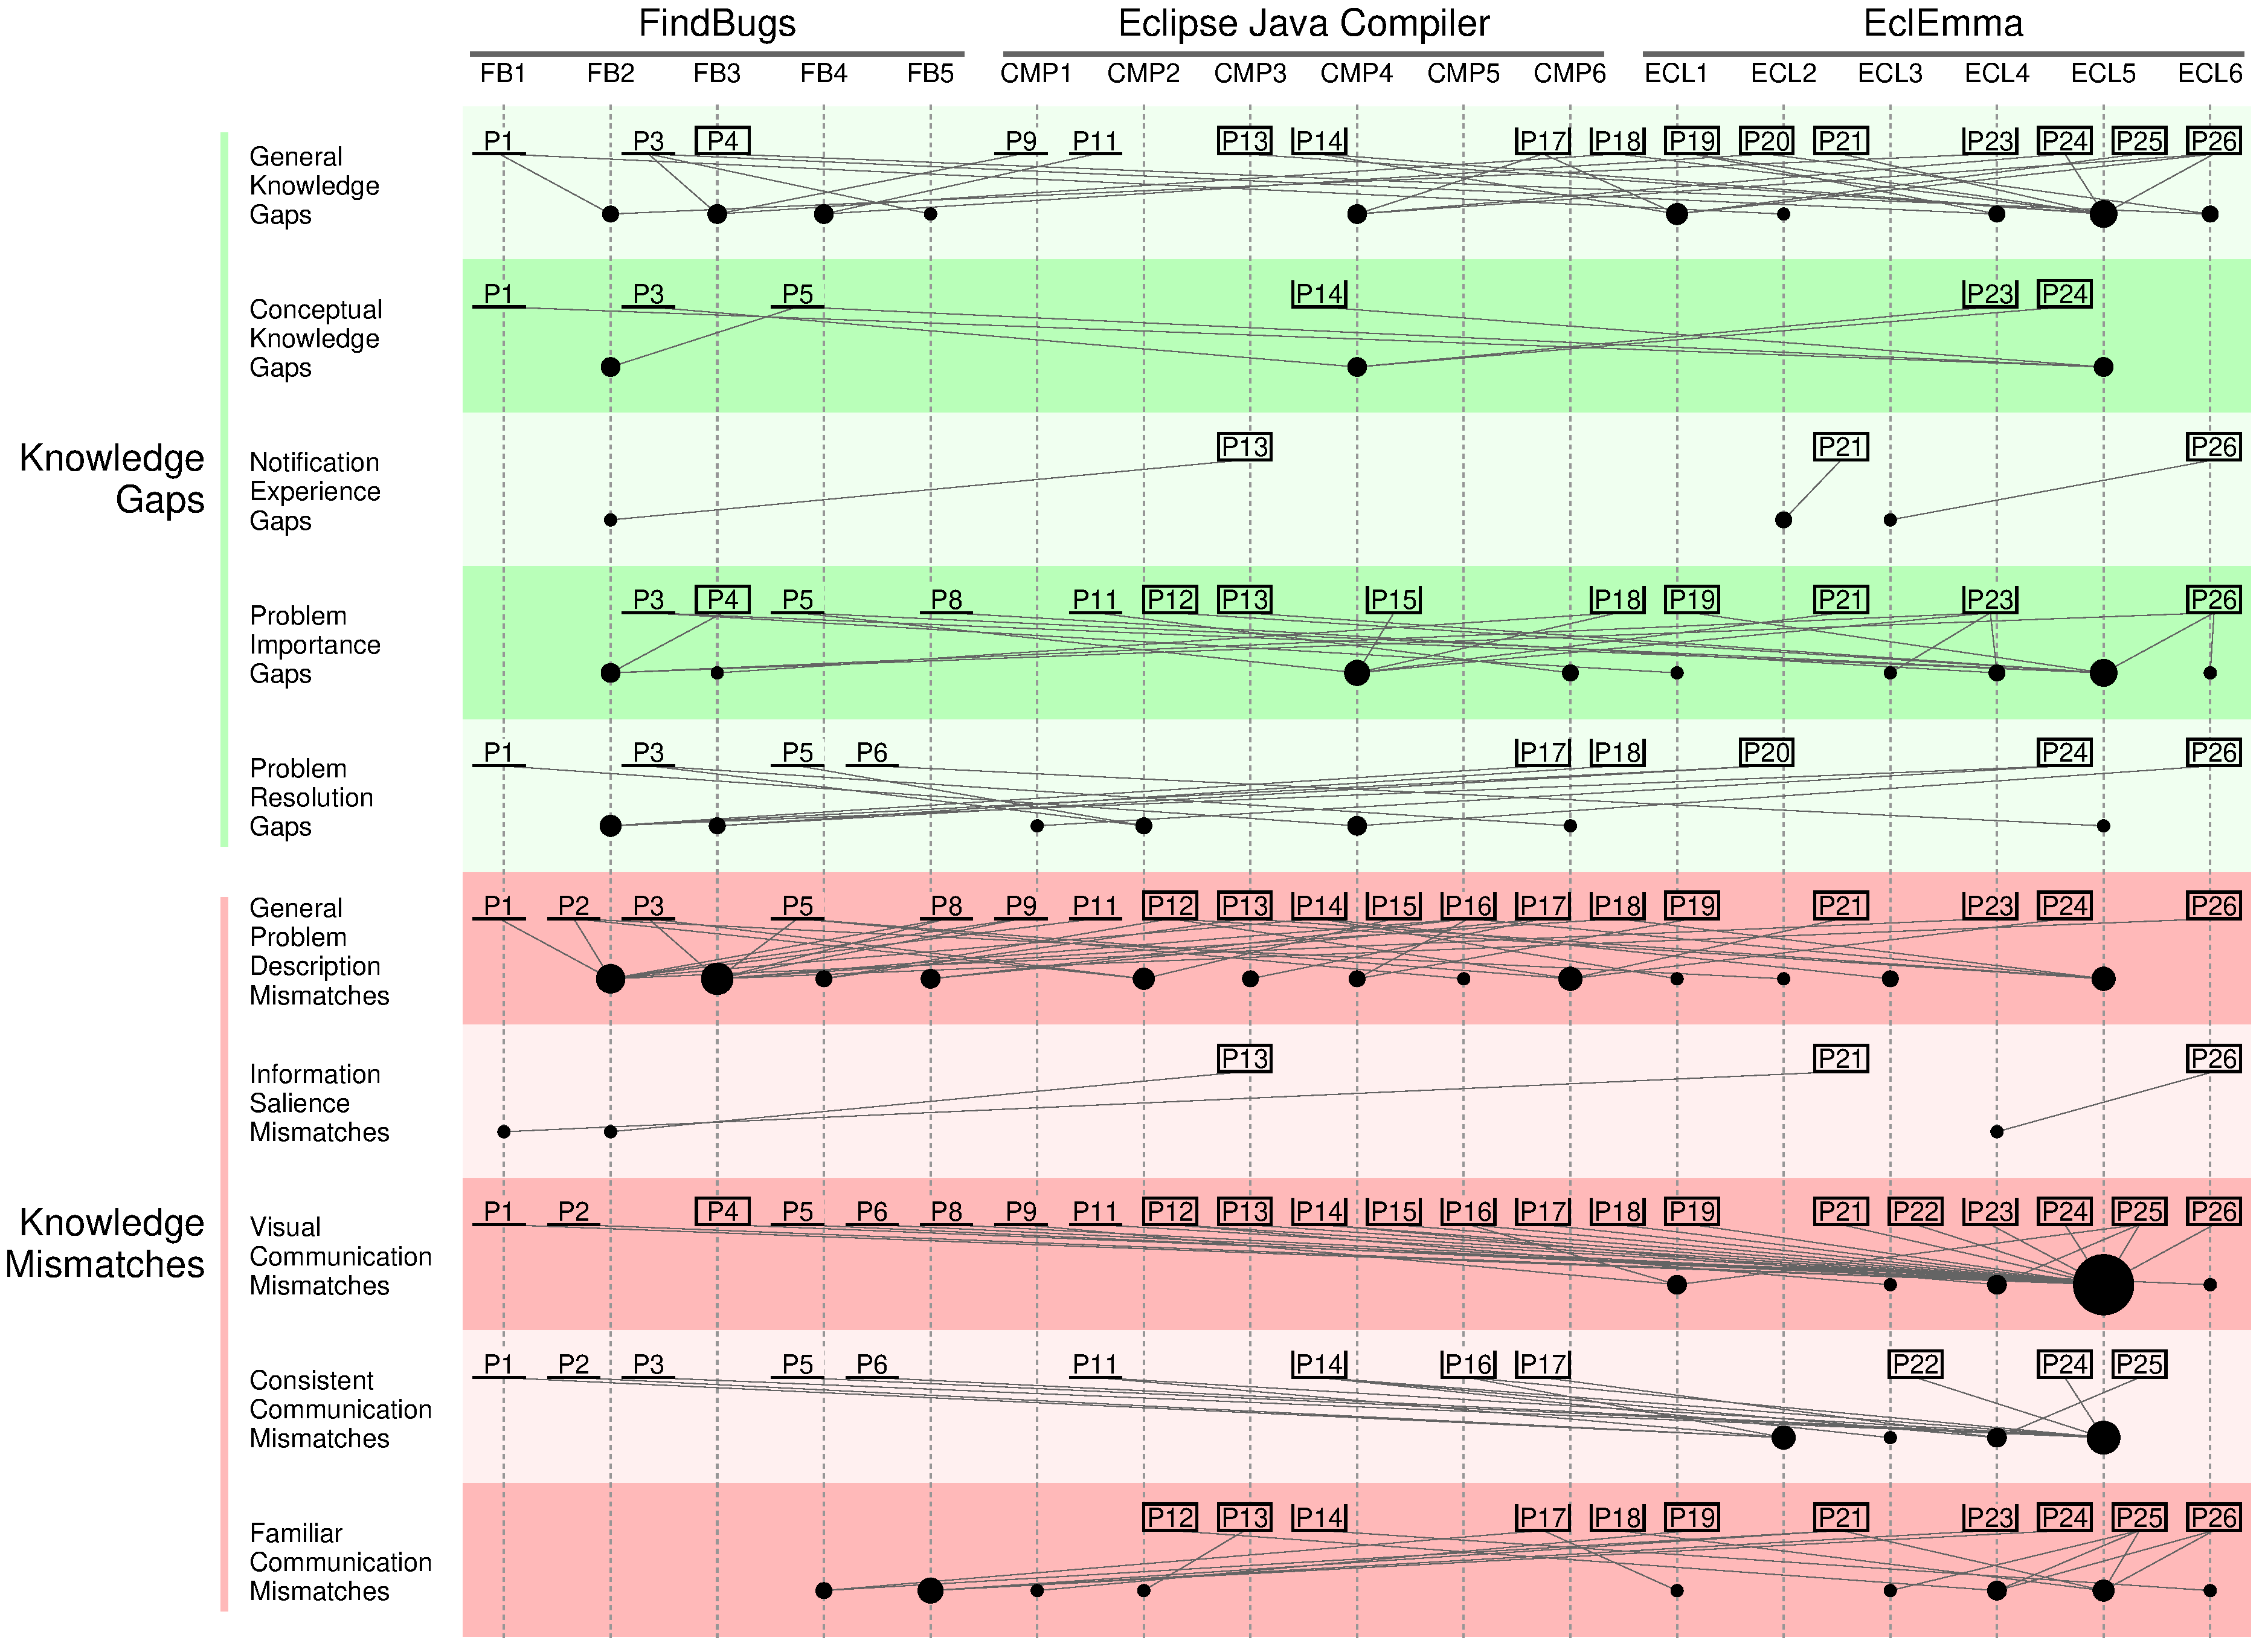
\includegraphics[width=\textwidth]{Chapter-4/figs/Issues_Full.pdf}};
	\end{scope}
	\begin{scope}[ocg={name=test1, ref=t1, status=invisible}]
		\node[inner sep=0pt] (svgPDF) at (0,0)
		{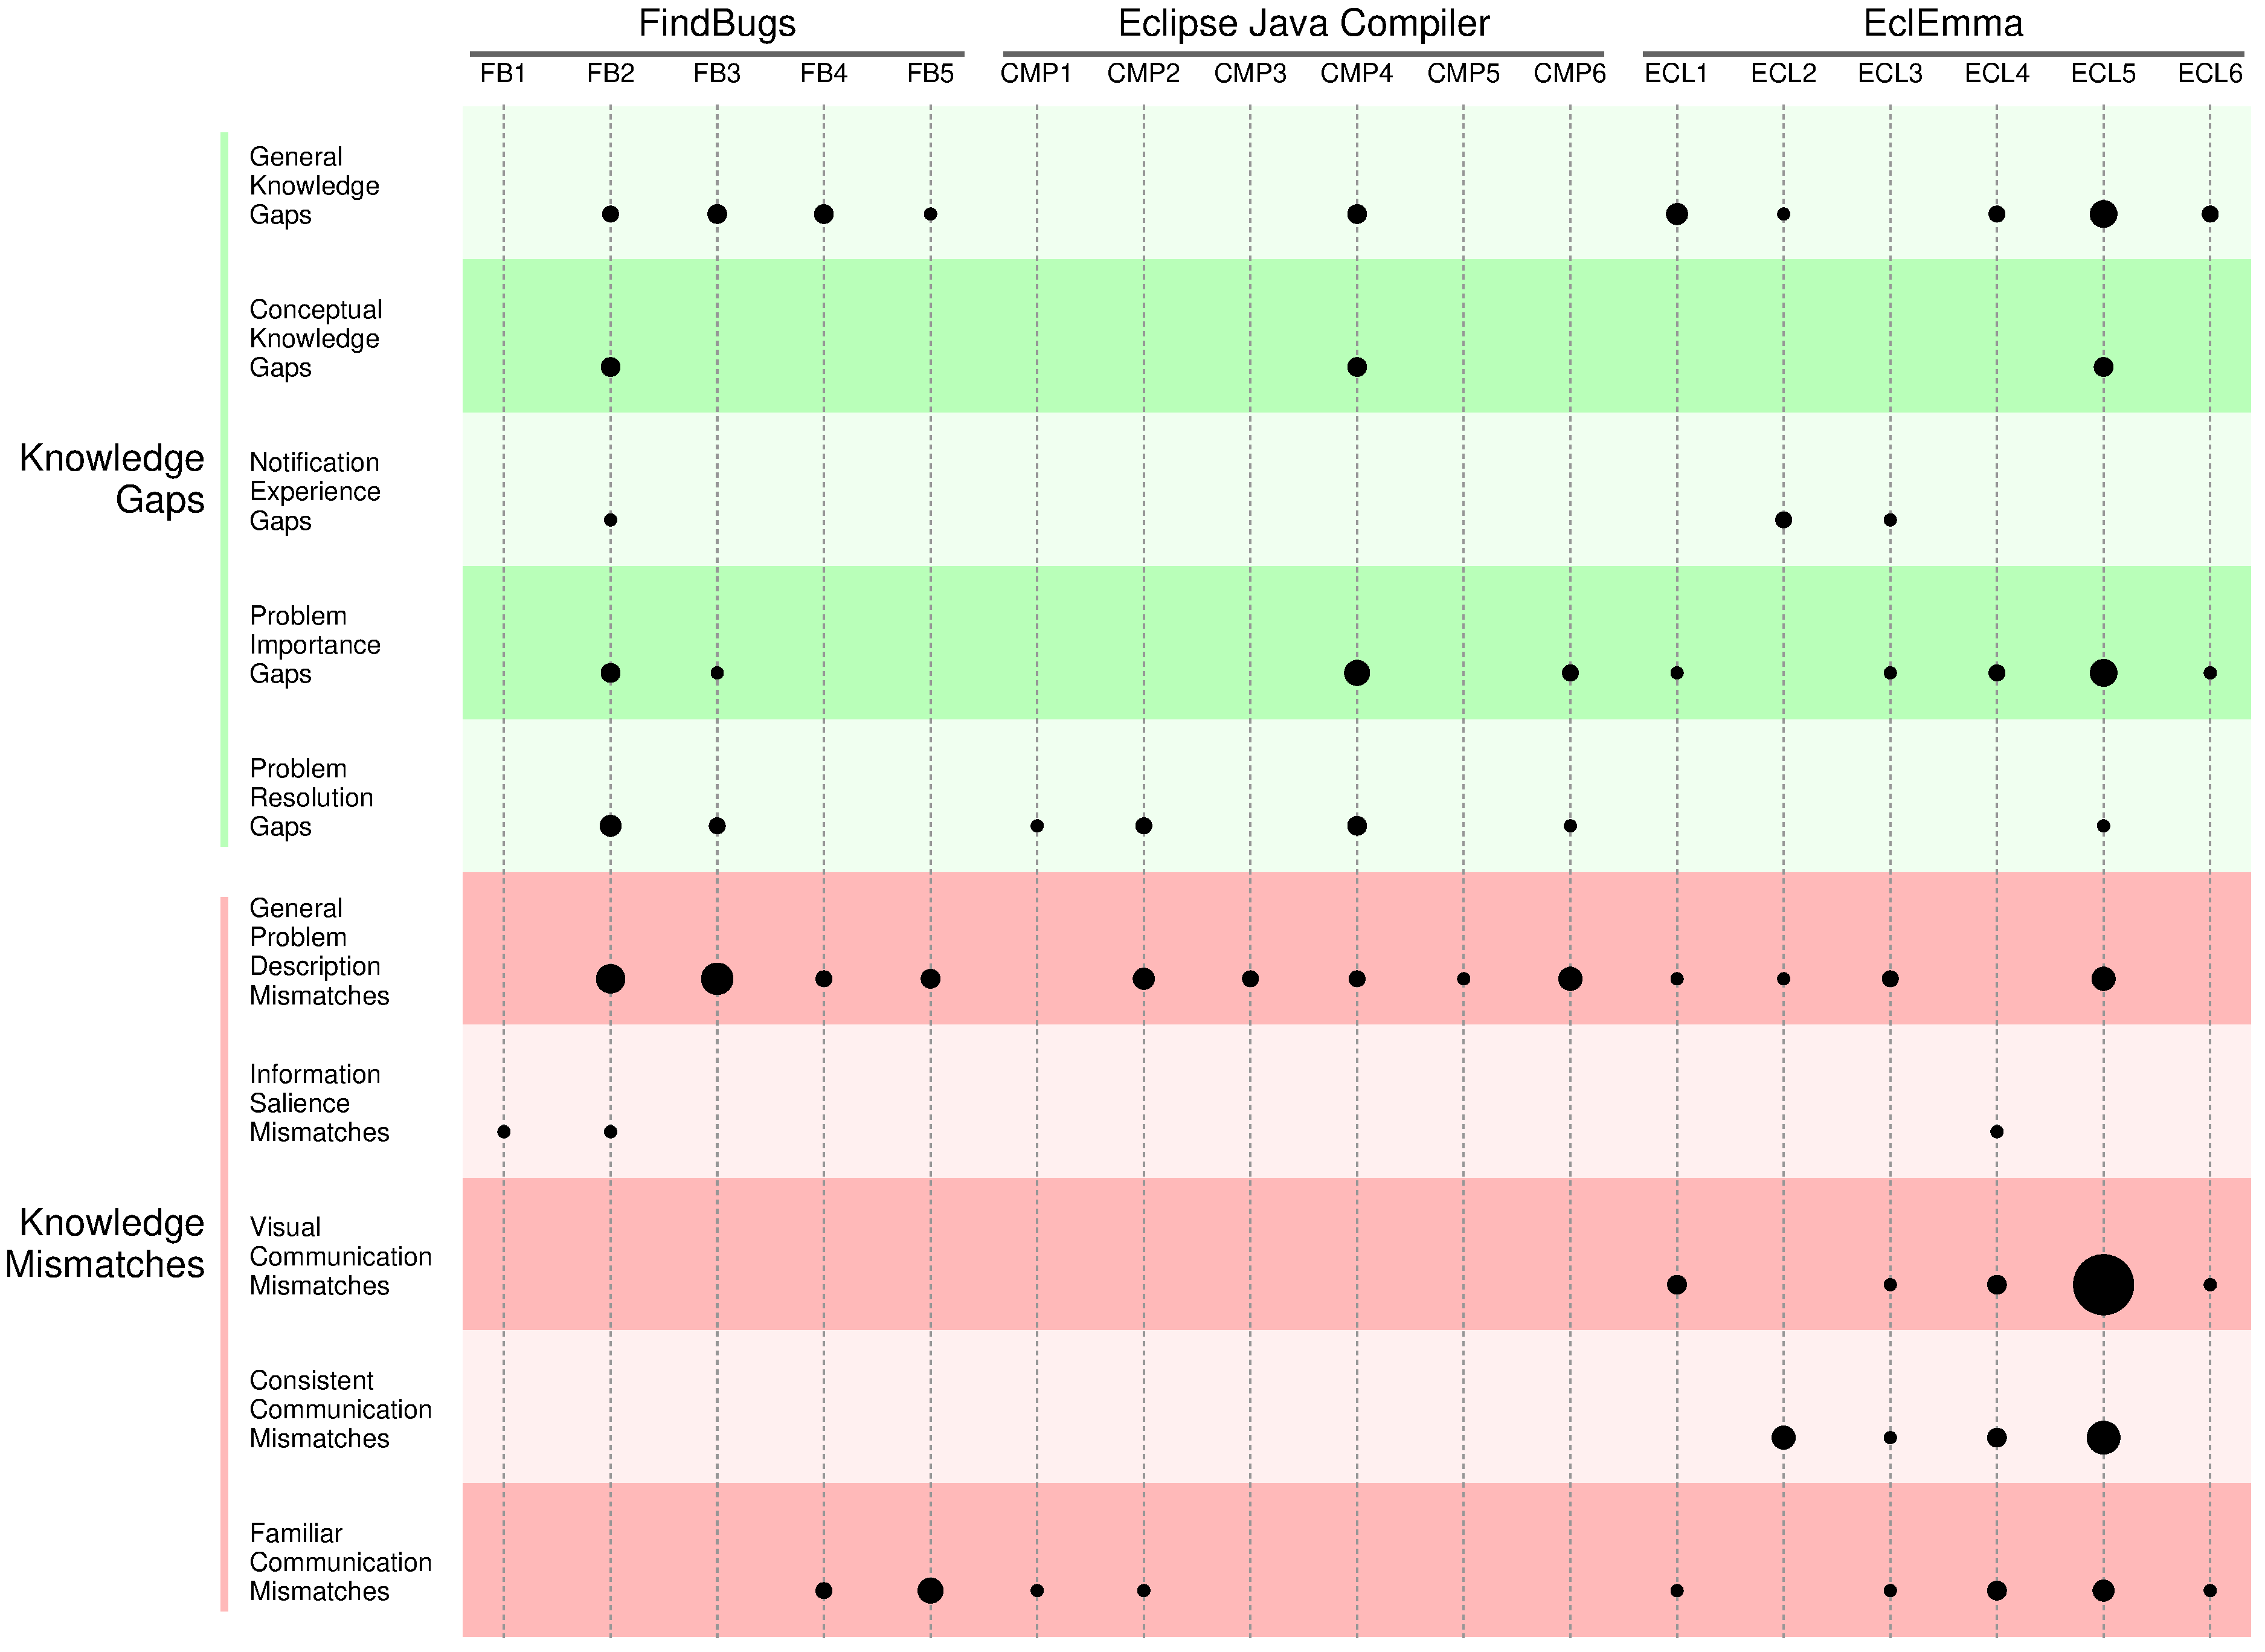
\includegraphics[width=\textwidth]{Chapter-4/figs/Issues_Challenges.pdf}};
	\end{scope}
	\node[draw,switch ocg={t1 t2}] at (0,-6.8) {Hide/Display Details};
}


%\begin{figure*}[ht] \centering \includegraphics[width=7in]{figs/results.pdf}
%\caption{Distribution of difficulties encountered and notifications that caused them.}
%\label{fig:results}
%\end{figure*}

\section{Knowledge-Related Challenges}

Remember Valerie from Chapter~\ref{chap-one}? Though she is a hypothetical developer, the challenges she faced are not hypothetical. Valerie experienced challenges caused by both knowledge gaps (no knowledge regarding lazy initialization) and knowledge mismatches (expecting an explicit connection to synchronization). 
Because research suggests experience matters when understanding vulnerabilities, and that experiences affect knowledge, I speak about knowledge here and throughout this thesis as the culmination of experiences~\cite{johnson1989mental,argote2011organizational,baca2009static}.
Using that definition, a \emph{knowledge gap} occurs when there is a gap between what the developer knows, based on her experiences, and how the tool communicates; a \emph{knowledge mismatch} occurs when what the developer knows and expects from the tool, based on her experiences, does not match the notification the tool uses.

% Based on this theory, I hypothesize that if it was possible for tools to be aware of what developers know and do not know, tools can improve communication by adapting its notifications to the developer.

\def\toggle{
	\begin{scope}[ocg={name=test2, ref=t2, status=visible}]
		\node[inner sep=0pt] (svgPDF) at (0,0)
		{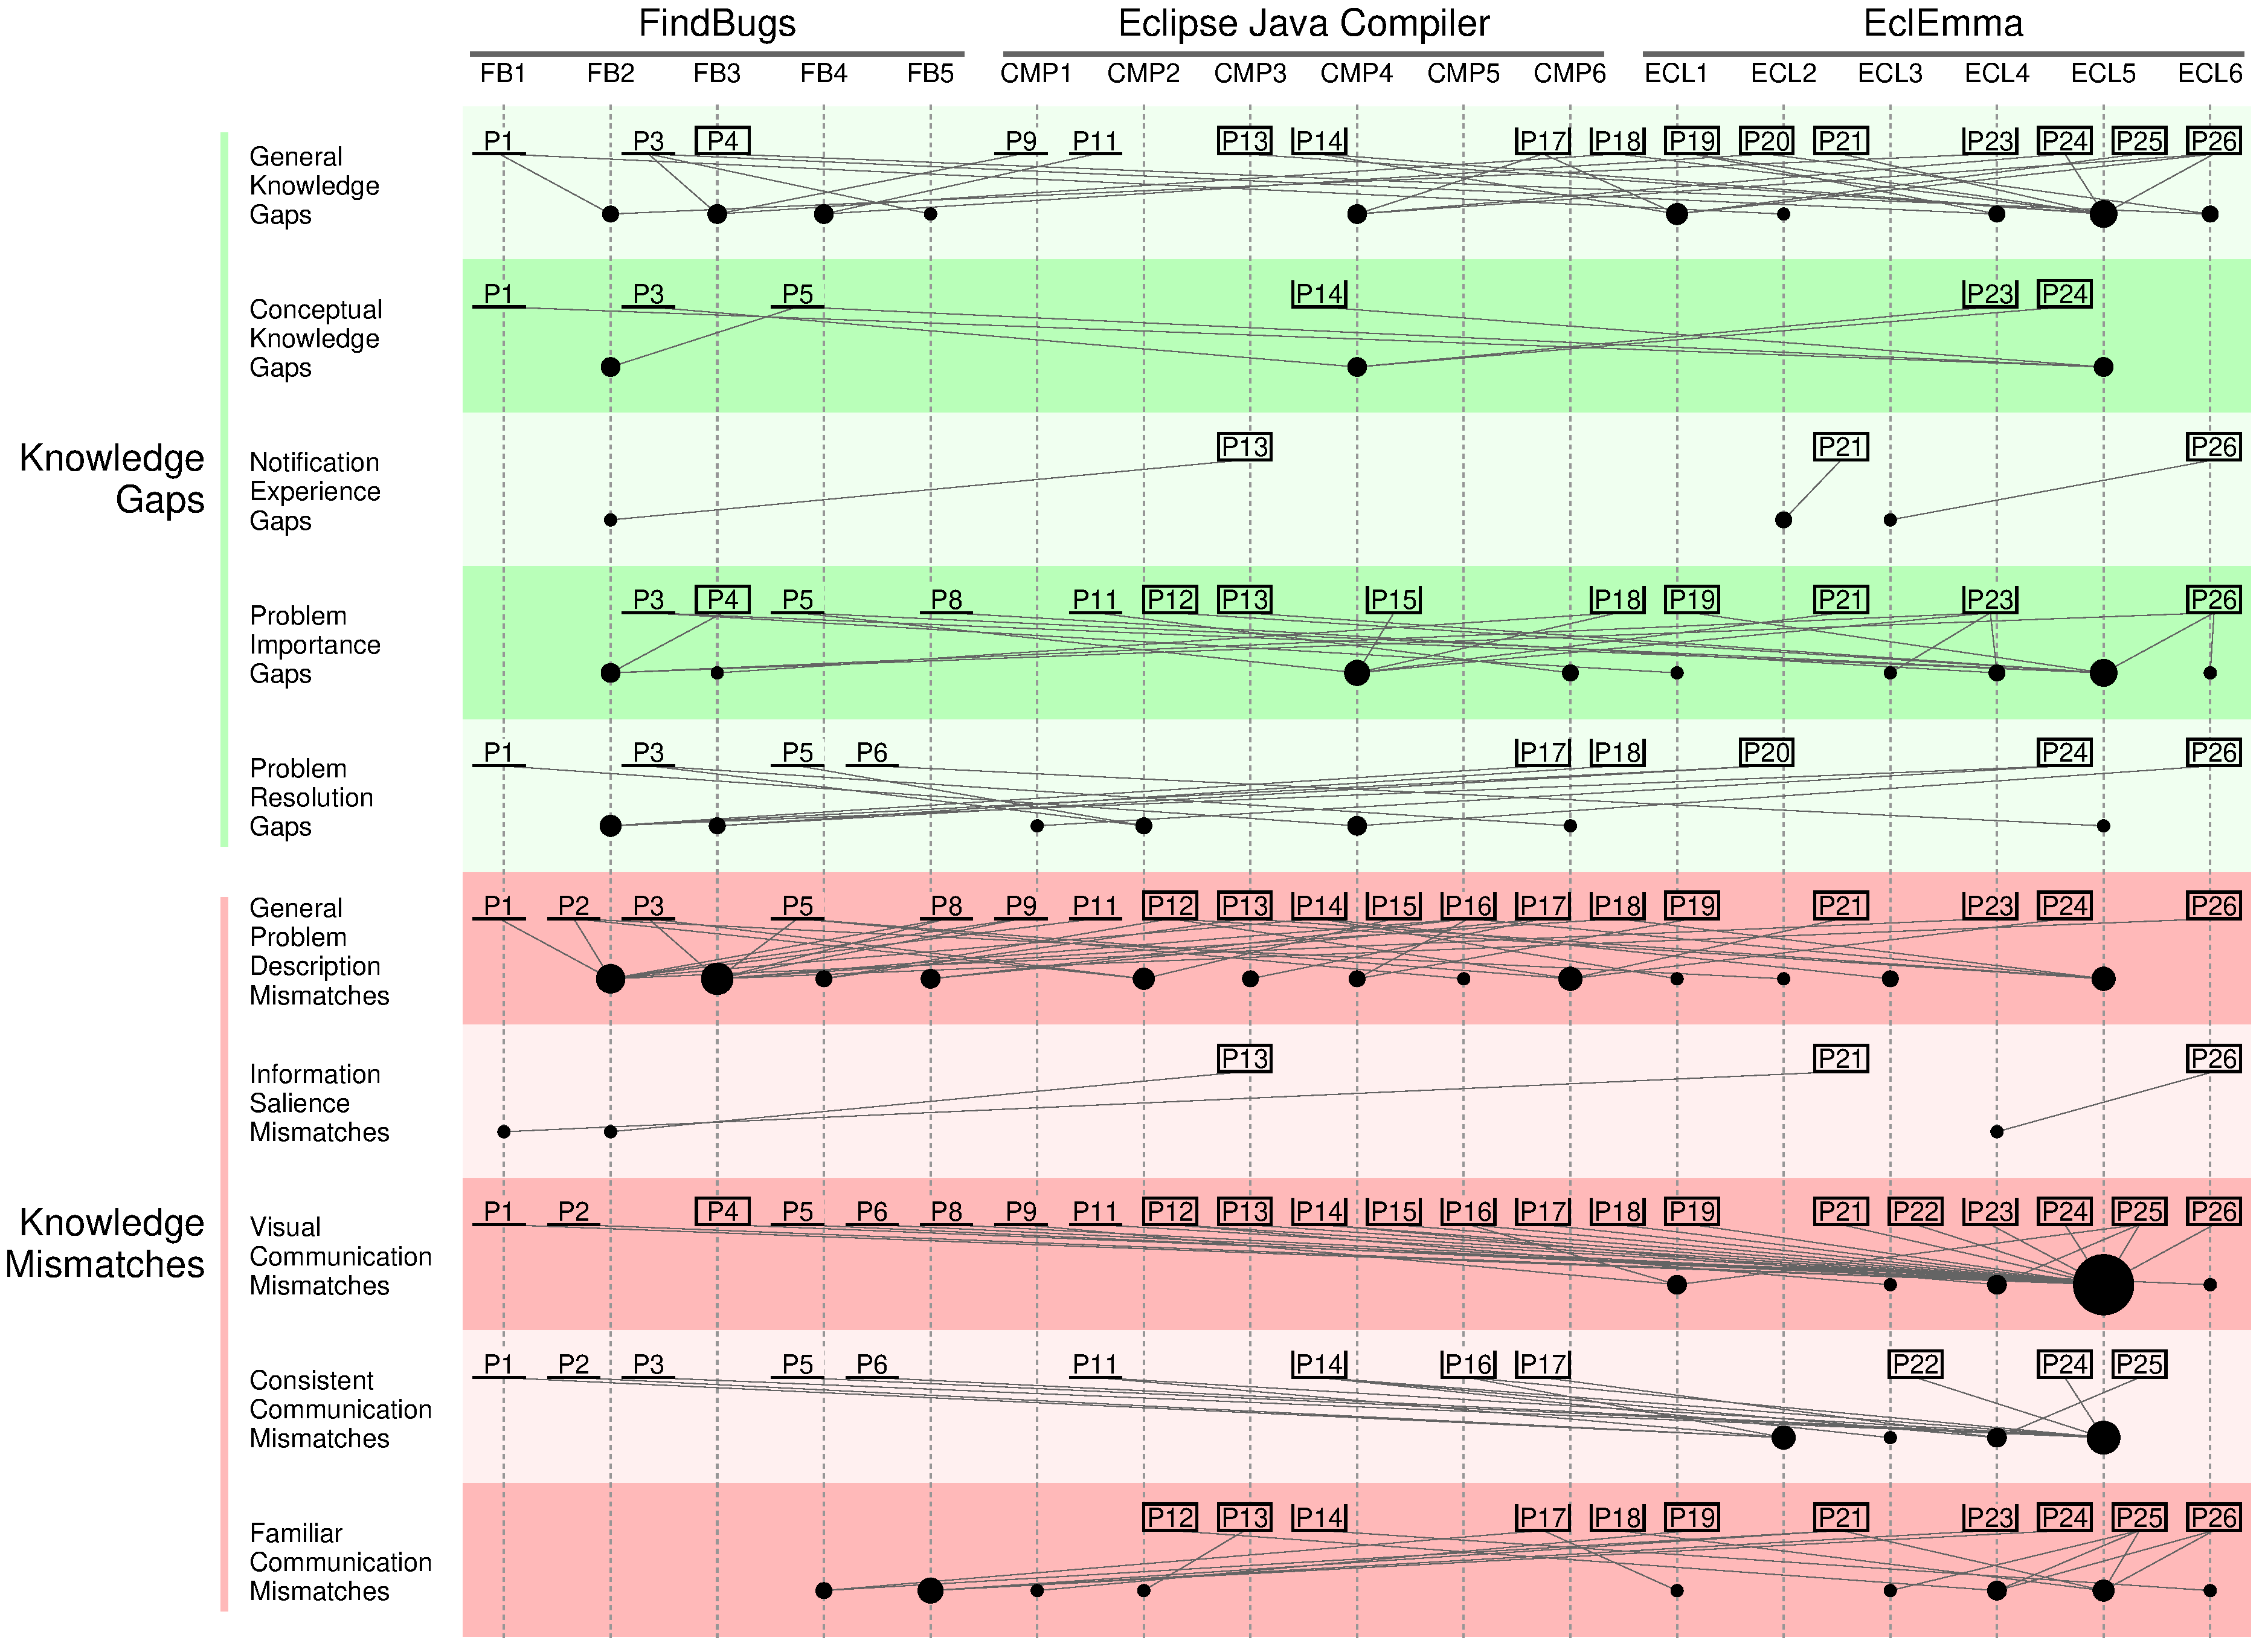
\includegraphics[width=\textwidth]{Chapter-4/figs/Issues_Full.pdf}};
	\end{scope}
	\begin{scope}[ocg={name=test1, ref=t1, status=invisible}]
		\node[inner sep=0pt] (svgPDF) at (0,0)
		{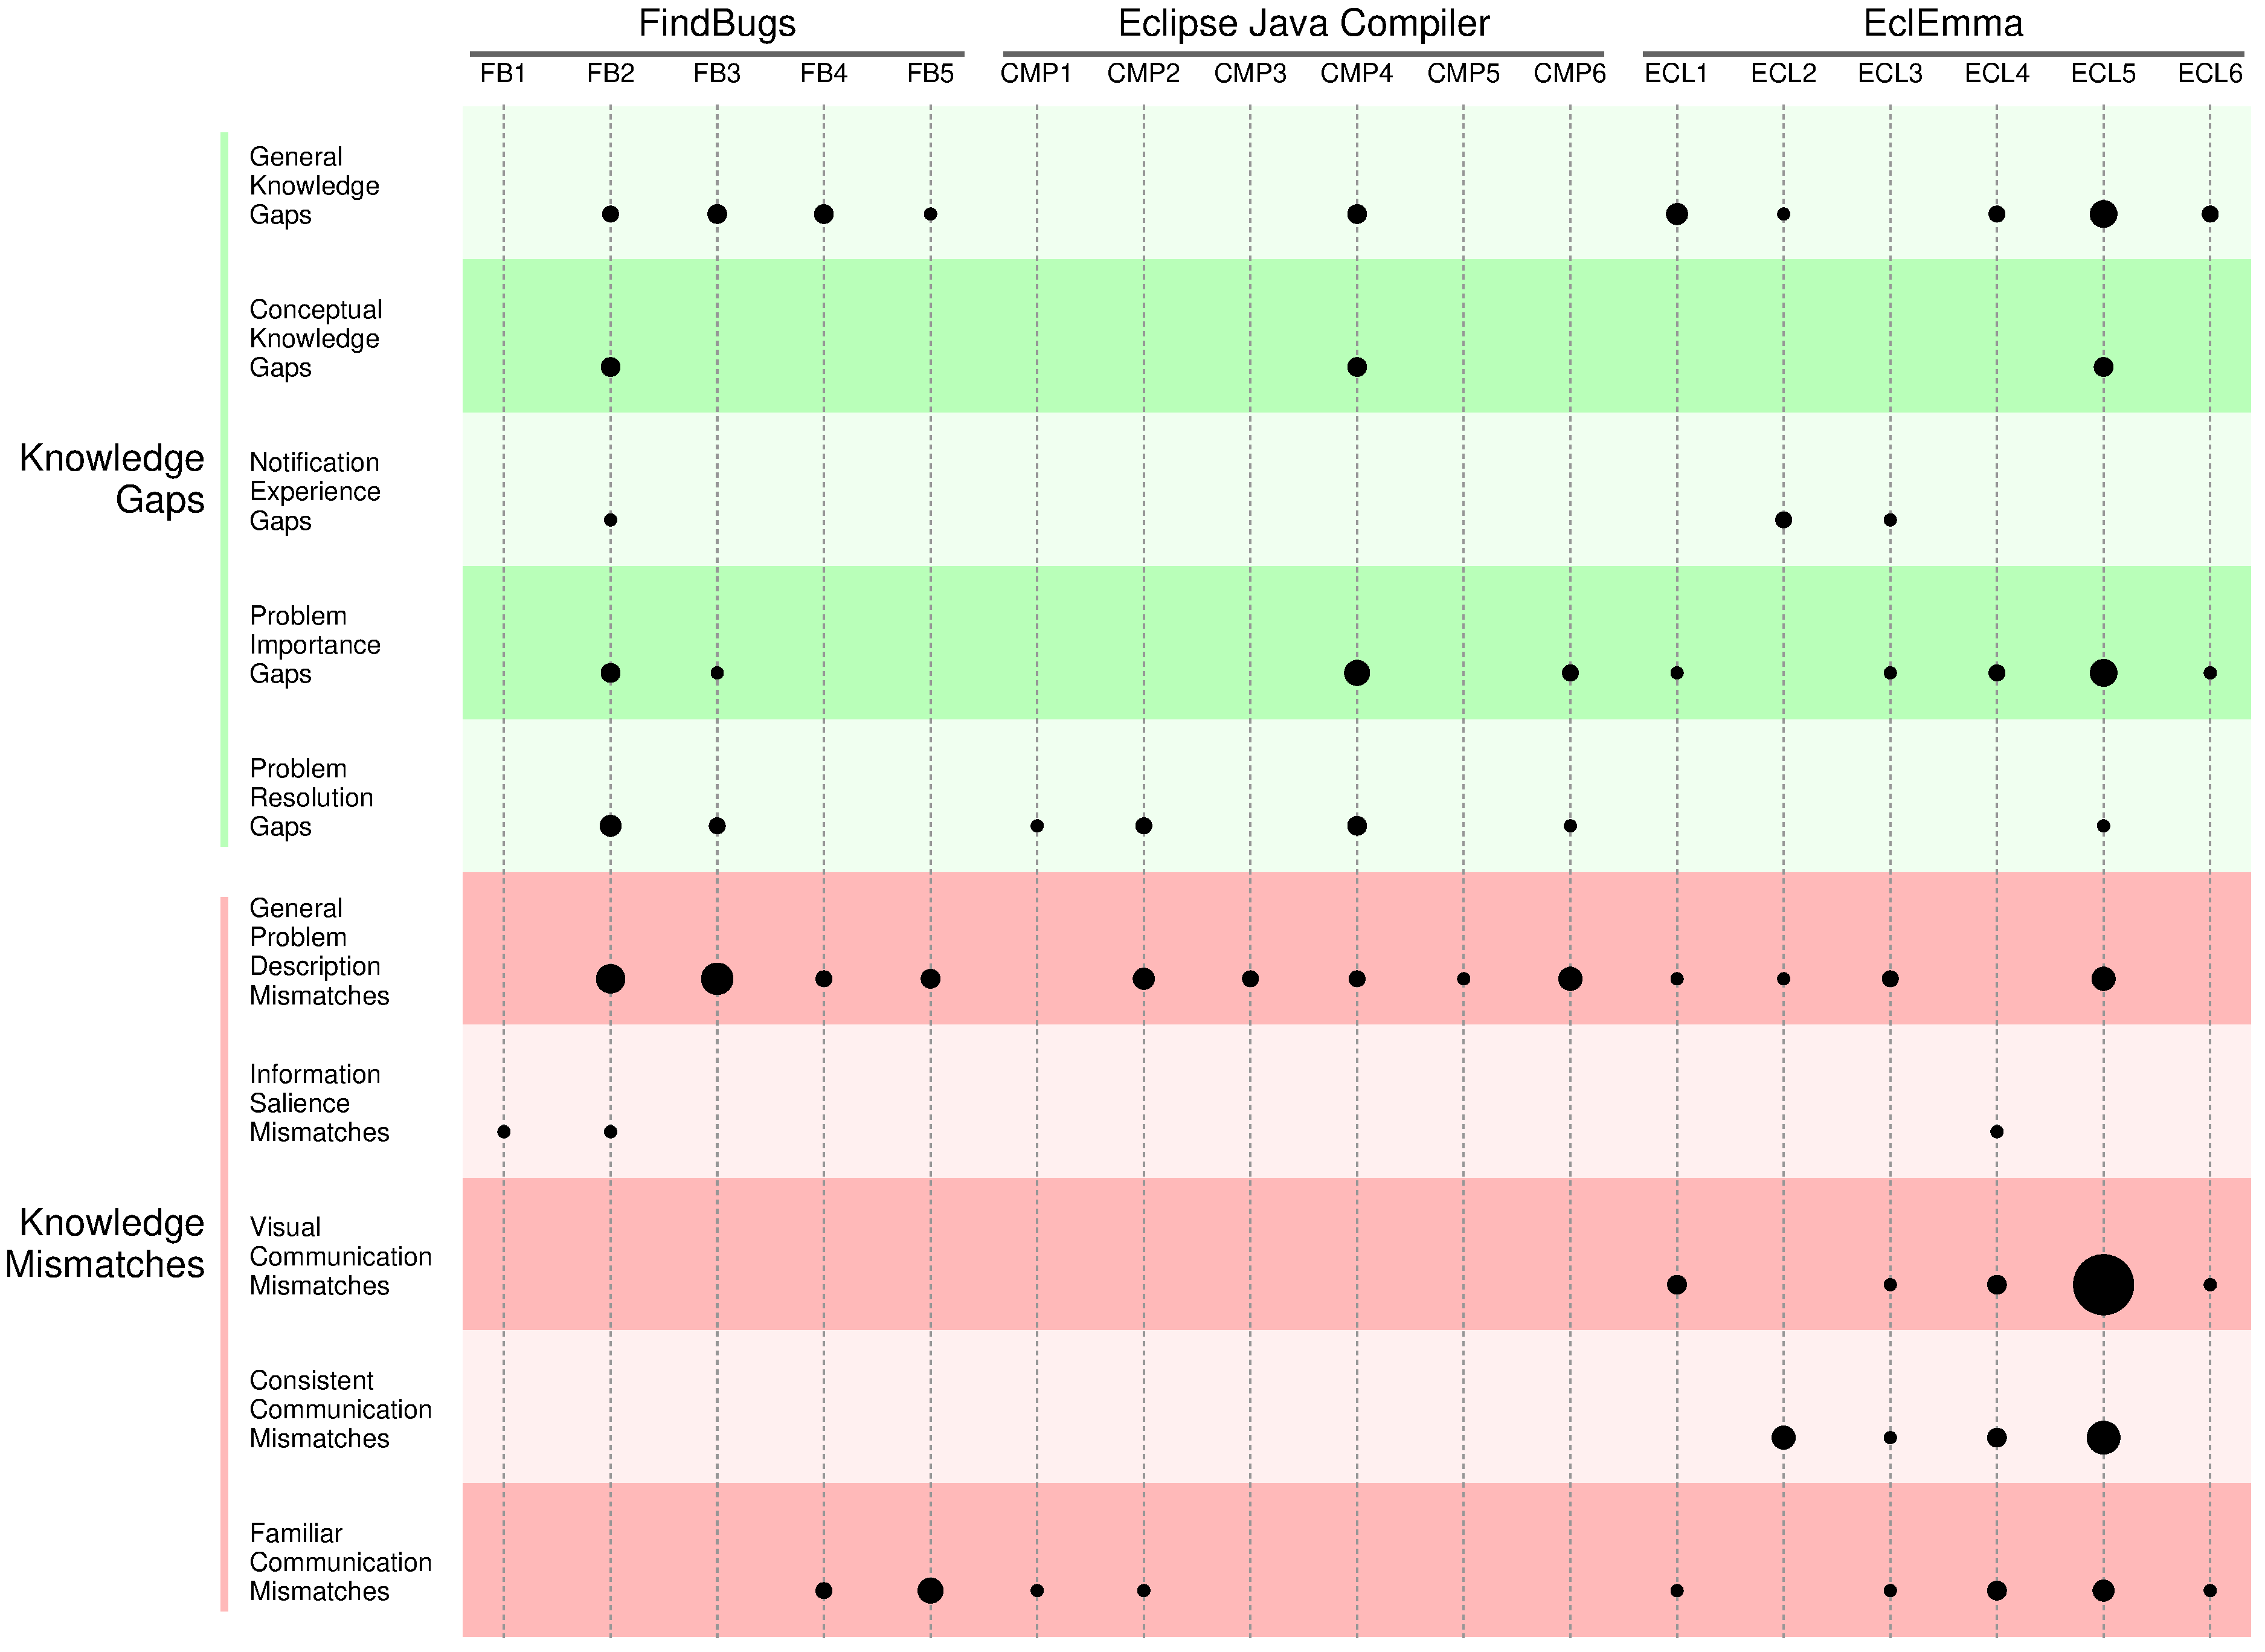
\includegraphics[width=\textwidth]{Chapter-4/figs/Issues_Challenges.pdf}};
	\end{scope}
	\node[draw,switch ocg={t1 t2}] at (0,-6.8) {Hide/Display Details};
}

\begin{figure*}[ht]
	\centering
	\begin{tikzpicture}
	\toggle
	\end{tikzpicture}
	\caption{Distribution of challenges encountered and notifications that caused them.}
	\label{fig:results}
\end{figure*}

The challenges that comprise my theory are 
shown in Figure~\ref{fig:results}.
Vertical lines represent the tasks and the horizontal bars indicate challenges.
The area of the dots indicate how many participants encountered challenges with that notification in that theme. 
Diagonal lines map participants to the challenges interpreting that notification.
\setlength\fboxsep{1pt}
When opened in Adobe Acrobat, clicking \framebox{``Hide/Display Details''} 
interactively toggles between showing and hiding this mapping.
I describe each challenge type, and validation of the findings, in detail in the remainder of this section.

\subsection{Knowledge Gaps}\label{subsec:gaps}

Knowledge gaps occurred when there was a gap between what participants know and the information provided by the notification. 
Knowledge gap challenges occurred when participants did not have existing knowledge of software 
development activities relevant to a given notification.  
However, we found it is not as simple as ``beginners battle and experts excel'', 
but instead that challenges faced by developers can occur regardless of programming or industry experience. 
In this subsection, I will describe general knowledge gap challenges, followed by four specific kinds of knowledge gaps identified in this study.

\subsubsection{General Knowledge Gaps}\label{subsec:infogap}
General knowledge gap challenges occurred when there was a gap between the general 
software development knowledge participants had relevant to the notification and the 
information provided by the notification.  
When participants did not provide enough information to map a challenge to a 
more specific kind of knowledge gap, I placed that challenge in this theme.
Participants experienced knowledge gap challenges across all three tools (Figure~\ref{fig:results}). 

FindBugs was more dominant in this theme than the compiler, with 9 and 2 participants encountering challenges respectively. This was the case, despite the compiler using less text than FindBugs to communicate. Participants focused on the text to understand the problem, but struggled to understand what the tool was trying to convey. Despite FindBugs' verbosity, as stated by 4 participants, the tool provided just enough to need to use the web to figure out the problem. For example, \professional{P25} struggled to interpret FB3. He made an effort to understand the notification, but then realized the notification did not provide enough for him to feel confident in his explanation, stating:

\vspace{0.5em}
\begin{quote}
	\textit{I would definitely want to correct it but I don't get enough info from here to know what to correct or what I did wrong so I would probably take this message and go to Google to see if anybody else is talking or saying something that I understand better.}
\end{quote}

\noindent
Participants who struggled with compiler and EclEmma notifications found themselves in a situation similar to \graduate{P17} when interpreting CMP4 and notifications in ECL1. When he encountered CMP4 and ECL1, he immediately realized the notifications did not provide enough information for him to come to a conclusion about each. He noted, like \professional{P25}, that he would need to use Google or documentation to better understand the notification being provided. \graduate{P17} was unable to come to a conclusion regarding either notification.
% some challenges that emerged clarify the types of information gaps developers may experience based on knowledge they have not, but would like to acquire

These findings confirm that more is not always better~\cite{Nienaltowski:2008:Compiler} for closing knowledge gaps and that these gaps exist with visual communication as well.
Along with general knowledge gap challenges, participants experienced challenges caused by four specific types of knowledge gaps that emerged: \textit{conceptual knowledge gaps}, \textit{notification experience gaps}, \textit{problem importance gaps}, and \textit{problem resolution gaps}.

\subsubsection{Conceptual Knowledge Gaps}\label{subsec:concept}
% challenge caused by no experience with concept
Conceptual knowledge gaps occurred when there was a gap between participants' knowledge of programming concepts, 
like serialization, present in the notification and the information provided by the notification regarding those concepts. 
\professional{P24}, a professional developer with 15 years of experience, attempted to work through 
CMP4 despite his unfamiliarity with serialization. 
His guess, based on the notification, was that he was missing a \texttt{serialversionUID}; 
however, beyond that he was unsure how a \texttt{serialversionUID} is associated with serialization. 
This led to the inability for \professional{P24} to fully interpret the notification.

\undergraduate{P5} encountered challenges interpreting FB2 due to conceptual knowledge gaps regarding multi-threading. 
The notification spoke about concepts such as lazy initialization, which \undergraduate{P5} noted he had not had past experience with. 
herefore, he could only guess what was wrong with the code.

Conceptual knowledge can also affect visual communication, even when the relevant concepts are not depicted in the notification. Test coverage is the obvious concept necessary to understand test coverage notifications. 
Some of the notifications participants encountered from EclEmma required knowledge of other concepts, such as exception handling. 
Three participants noted they could not confidently explain EclEmma notifications involving \texttt{finally} blocks using the visuals provided due to their minimal experience with \texttt{finally} blocks.

After completing ECL5, most participants could at least vaguely explain the notifications they encountered. 
However, \undergraduate{P5} still could not definitively conclude anything about the notifications, stating: 

\begin{quote}
	\textit{I don't know what \texttt{finally} means but it seems like everything inside \texttt{try} 
	is not getting called\ldots I assume \texttt{finally} is similar to \texttt{catch} 
	but I don't really know how \texttt{finally} works.}
\end{quote}

\noindent
His lack of knowledge regarding \texttt{finally} blocks made it challenging for \undergraduate{P5}, 
despite his familiarity with other relevant code structures\footnote{The reader may also find this confusing, but this was a design decision made by EclEmma's toolsmiths. This confusion arises from a difference between the bytecode representation and the source code representation of \texttt{finally} blocks (\url{https://github.com/jacoco/jacoco/issues/15}). Although this may seem like a design problem, we included the notifications we did, including ECL5, because they are encountered in the wild.}. 
This, coupled with being his first experience with EclEmma notifications, led to his inability to interpret the notifications in ECL5.

\subsubsection{Notification Experience Gaps}\label{subsec:notif}
Notification experience gaps occurred when there was a gap between participants' knowledge gained 
from experience with a notification they encountered for the first time and the notifications they have previously encountered. 
Participants' lack of experience with a notification is the knowledge gap that caused challenges in this theme.
For example, \graduate{P21} struggled to interpret the notifications in ECL2 due to the differences in highlighting on uncovered methods and constructors.  His comments suggested that he understood the concept of coverage, but stated that the challenge was due to unfamiliarity with the tool.
When he first encountered an uncovered method notification, without the signature highlighted like a constructor's signature was, he could not determine whether \emph{lack of highlighting} was equivalent to \emph{red highlighting}.
The challenges in this theme are general in that they relate to overall notification knowledge. Some of the challenges that emerged relate to gaps in knowledge regarding notification specifics, such as importance and resolution. 

\subsubsection{Problem Importance Gaps}\label{subsec:rationale}
% challenge caused by don't know why they should care or why they should resolve, and not mentioned in notification
Problem importance gap challenges occurred when there was a gap between participant knowledge of the importance of the problem and the notification's attempt to communicate importance.
As \graduate{P18} attempted to explain FB3, he realized that although the notification did tell him that he was synchronizing on a mutable field, it did not tell him why that is undesirable. 
He attempted to determine a reason for why it is undesirable, and though he found the notification's message ``unlikely to have useful semantics'' helpful, he noted that his reasoning ``would not be correct'' because he would have to guess.

Without an understanding of why the problem was bad, participants could not confidently interpret the notification; this led to challenges coming up with resolutions. 
For example, \undergraduate{P5} could not confidently resolve CMP4; the notification was clear that a missing \texttt{serialversionUID} is the problem, but did not specify why the ID was needed. 
Though the compiler provided quick fixes, deciding which fix was best for \undergraduate{P5} depended on what the ID was used for, which the notification did not specify.

\subsubsection{Problem Resolution Gaps}\label{subsec:resolution}
Problem resolution gap challenges occurred when there was a gap between what the participant knows about resolving a notification and the resolution suggested by the notification. Most often this gap was present because the notification did not include information specific to notification resolution.
When participants did not know how to fix a notification, they had to guess how they might fix it or, as \professional{P20} noted, ``Google it to make sure'' they fully understood the notification and how to fix it. 
The downside to this approach is that it takes developers into a form of information foraging that involves leaving their working context~\cite{Altmann:2004:Task}, which \professional{P13} explicitly stated:

\begin{quote}
	\textit{Anything that deviates my train of thought from the task at hand\ldots that's the last thing you want when writing code.}
\end{quote}

\noindent
The notifications that did provide a fix description did not provide a clear description of the fix or how to apply it; without the required knowledge, filling this gap was difficult for participants.
This was most often the case with the compiler, which provides quick fixes with minimal explanation attached.
Two participants struggled with understanding and resolving CMP4. Both appeared confident that something was missing and that they should add the \texttt{serialversionUID}. However, neither knew what a \texttt{serialversionUID} was or how they should have used it. 

Sometimes notifications provided multiple options for resolution but did not provide information regarding which resolution was most appropriate. This left participants with the task of determining the best fix to apply. For example, CMP4 offers multiple fix possibilities, each with its own set of code changes and possible side effects. \professional{P26} spent time sorting through and discussing the options for fixing CMP4. Because the tool did not provide information regarding the pros and cons of a each fix, he was unable to explain how to resolve the notification.

\subsection{Knowledge Mismatches}\label{subsec:mismatch}

Knowledge mismatch challenges occurred when there was a mismatch between how participants expected a notification to communicate, based on their knowledge, and how the notification communicated.
Unlike knowledge gap challenges, participants had knowledge relevant to the notifications and concepts. However, they encountered  challenges when attempting to use their knowledge to interpret the notification. 
As with knowledge gaps, I describe general mismatch challenges, followed by discussion of four specific kinds of knowledge mismatches identified in this study.  

\subsubsection{General Problem Description Mismatches}\label{sec:description}
General problem description mismatches occurred when there was a mismatch between the way the participant would textually describe the problem and the description provided by the notification.
Although other challenges relate to notification text, for General Problem Description Mismatch challenges, it was unclear what about the description participants found confusing.  
However, it was clear that the text was not communicating in a way that participants could use their knowledge to reconcile.
This is related to research on compiler messages conducted by Traver that suggest unambiguity of language is important~\cite{Traver:2010:Messages}.
Similarly, O'Neil discussed the importance of language considerations in data breach notifications~\cite{o2015target}.

Representative of textual communication mismatch challenges was \graduate{P16}'s experience interpreting FB5. After he read the text provided by the notification, \graduate{P16} was unable to come to a definite conclusion regarding the problem, stating:

\begin{quote}
	\textit{It didn't confirm or deny what I thought because the wording of the [tool tip] was not quite how I would have described it\ldots}
\end{quote}

\noindent
Participants encountered similar challenges with the compiler. \graduate{P17}, for example, went back and forth between the text of CMP3 and information provided via quick fixes as he tried to understand the problem. 
He was able to guess, based on his knowledge, what the problem might be but moved away from the text of the notification to come to any sort of conclusion about the problem being communicated.

For some participants, the language notifications used was familiar but not something they could quickly recollect. 
\undergraduate{P3}, for example, saw the word ``mutable'' in FB3 and he could not remember what mutable meant.
After \undergraduate{P5} read the text provided for FB3, he explained that the use of the phrase 
``useful semantics'' may not have been the best choice as, for him, terms like this ``have different meanings 
in computer science and the real world.''

Similarly, \undergraduate{P5} and \professional{P24} struggled due to ambiguity in the language used.
\undergraduate{P5} found the overall phrasing of CMP6 ``weird.'' 
\professional{P24} was more specific in stating how the language was ambiguous. 
He found the use of the word ``applicable'' to be odd in this context and not clearly indicative of the message he assumed 
the tool was trying to communicate. 

Although these textual mismatch challenges encountered are general, specific types of mismatches with the text portion of the notification emerged: \textit{information salience mismatches}, \textit{visual communication mismatches}, \textit{consistent communication mismatches}, and \textit{familiar communication mismatches}.

\subsubsection{Information Salience Mismatches}\label{subsec:buried}
Information salience mismatches occurred when there was a mismatch between the information a participant thought was most relevant and the information the notification made salient. 
This aligns with McCrickard and Chewar's suggestion that general computer users are dissatisfied with notification systems because of mismatched information prioritization~\cite{mccrickard2003attuning}.

Representative of these challenges was~\professional{P13}'s attempt to interpret FB2 (Figure~\ref{fig:N2}).~\professional{P13} read the tooltip for FB2 but did not find anything useful; he saw ``update of static field'' but was not certain what the tool was trying to communicate. 
After digging deeper, he found that the tool eventually elaborated on what is wrong with where and how a field is set when working with threads. 
This was what he was looking for, as it helped him understand why it was a ``\emph{very serious} multi-threading bug,'' as the notification stated. 
For him, and the other participants who encountered challenges in this theme, the most easily available information was not so useful, leaving them unsure of what the problem was in the code and why it was a problem. 
The critical pieces of information, such as that it is a multi-threading problem concerning where synchronization is placed, got buried.

I only observed this phenomena with more experienced developers; this suggests that more experienced developers may have more concrete expectations of what information tools should provide.
On the flip side, less experienced developers may not know when important information is buried because they are unsure of what the important information is. Therefore, less experienced developers did not appear to encounter challenges in this theme.

\vspace{1.5em}

\subsubsection{Visual Communication Mismatches}\label{subsec:expectations}
% participants have experiences that suggest how problems should be communicated but encountered challenges when those expectations were not met (general)
% talk about General Description issues here??

\begin{figure} \centering 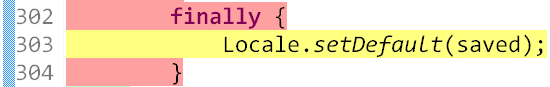
\includegraphics[width=2.5in]{Chapter-4/figs/finally-block}
	\caption{A notification from EclEmma regarding \texttt{finally} coverage (ECL5).}
	\label{fig:finally}
\end{figure}


Visual communication mismatches occurred when there was a mismatch between how the participant would communicate with other developers about the notifications and the visual elements used by the notifications.
For these challenges, it was clear there was a mismatch between what participants expected and what the tool presented them with, but there was no indication by participants of what specifically caused the mismatch.

For fourteen participants, EclEmma's attempts to communicate \texttt{finally} block coverage in ECL5 (Figure~\ref{fig:finally}) failed because it was not obvious, based on their mental model of how \texttt{finally} blocks work, how a \texttt{finally} block can be missed or the code inside a \texttt{finally} block could be partially covered. For example, \professional{P24} had expectations regarding how EclEmma might communicate coverage of a \texttt{finally} based on prior experience with the construct that suggests it always executes. Rather than exploring more, \professional{P24} noted he did not understand the way the tool communicated. 

Seven participants had expectations regarding how \texttt{try} blocks work that did not match how EclEmma reported \texttt{try} block coverage (ECL5).
For example, as \graduate{P23} sorted through the notifications in ECL5, he wanted to know which line failed to cause the \texttt{try} block to not execute.
Attempting to interpret the notification, he stated:

\begin{quote}
	\textit{In order for the \texttt{catch} statement to be activated I would imagine that this code had at least been evaluated.}
\end{quote}

\noindent
His expectation, based on his knowledge of the code construct, was that if the \texttt{try} did not execute, there was a line of code at fault. However, contrary to his expectations, EclEmma highlights the entire \texttt{try} block red if an exception is thrown, which makes it unclear whether the \texttt{try} executed at all, and if it did, where an exception was thrown.

Five participants got confused by EclEmma's lack of textual information.
Participants probably noticed this because both FindBugs and the compiler provide supplemental textual information when markers, similar to the ones provided by EclEmma, are clicked; in fact, markers and notifications from other tools within EclEmma's interface sometimes distracted participants looking for information regarding code coverage.
As \professional{P4} accessed the information provided by notifications in ECL6, he noticed and explored the availability of multiple markers that provided information. Some of these markers came from other tools; none provided \professional{P4} with ``any details about the coverage part,'' so he was not sure why they were present.

%These expectation mismatch challenges are general and focus on visual communication. Participants also encountered related, but more specific knowledge expectation mismatch challenges.


\subsubsection{Consistent Communication Mismatches}\label{subsec:inconsistent}
% challenges caused by tool communicating similar problems differently
Consistent communication mismatches occurred when there was a mismatch between the consistency expected by the participant and the inconsistencies in how the notifications communicated similar problems. 
Prior research suggests that within-tool-consistency is an important factor for developers when interpreting and addressing compiler messages~\cite{Traver:2010:Messages}.
The results in this category suggest that experiences affect perception of consistency and that this phenomena generalizes to visually-enriched notifications in other types of  tools.

Five participants encountered challenges caused by inconsistencies in how EclEmma reports coverage on branching structures. Under the assumption that yellow highlighting was accompanied by a textual description (i.e. 1 of 2 branches missed), participants often struggled to interpret notifications like the one in Figure~\ref{fig:finally}. \undergraduate{P6}, among others, spent a significant amount of time during her session trying to interpret the notifications in ECL5. When she realized that there were no markers available to better explain partial coverage inside a \texttt{finally} block, she began looking at the other similar notifications in ECL5. When she realized that none of the other notifications had what she was looking for, she summarized why she was struggling, stating ``I'm not sure what the other option could be\ldots it doesn't have the little yellow diamond on it.''

Six participants noticed inconsistencies in how EclEmma reported coverage on non-branching code structures. Five of the six encountered challenges interpreting notifications on methods and constructors. 
EclEmma highlights the constructor signatures to indicate a missed constructor, however, does not highlight a method signature when it is not executed. 
For example, during \professional{P14}'s session, he did a lot of back and forth between EclEmma tasks to compare notifications. As he tried to interpret the notifications in ECL3, he reflected on and revisited ECL1 and ECL2, where he recalled there being class, method, and constructor coverage. He remembered the inconsistencies with how ECL1 and ECL2 communicated coverage on these constructs and found it to be confusing. Therefore, he could not give a definite interpretation of any of the three. 

\subsubsection{Familiar Communication Mismatches}\label{subsec:intuitive}
% challenges caused by unintuitive communication; participants explicitly noted the notifications as being unintuitive
Familiar communication mismatches occurred when there was a mismatch between participant familiarity with the methods a notification uses to communicate about programming concepts and the methods the notification used to communicate about programming concepts When participants encountered these challenges, they often noted lack of familiarity or the inability to easily recognize the problem.
%color representations - P12, P15, P18, P21, and P24
Participants that noticed unintuitive communication techniques found some for all tools. The majority of participants (five of eleven) stated that EclEmma's dominant use of color to communicate code coverage was not intuitive. For example, participants did find it intuitive to use yellow for partial coverage in notifications like the ones in ECL3, ECL5, and ECL6. 
The common problem with the other tools involved association of the notification to the root cause and unintuitive fix descriptions.

\subsection{Member Check}
To assess the validity of how I interpreted the data, and the experiences developers have when interpreting tool notifications, we conducted a member check. Of the seven responses received, two developers agreed with these findings and five strongly agreed. Many found the report ``interesting,'' some noting that although they may not have experienced all of the challenges during the study, they can recall previously encountering such challenges. When asked which challenges they can relate to the most in their experiences with tools, the most common choice was Problem Resolution Gaps (5). The second most common responses (4) include Notification Experience Gaps and Information Salience Mismatches, followed by the third most common responses (3) of Conceptual Knowledge Gaps, Visual Communication Mismatches, and Familiar Communication Mismatches.

\section{From Theory to Practice}
Current tools do not support developer knowledge gaps (Section~\ref{subsec:gaps}) and sometimes conflicts with existing developer knowledge (Section~\ref{subsec:mismatch}).
In this section, I discuss several implications of the findings from this study.

\subsection{Filling Developer Knowledge Gaps}
Despite the experience of some participants, every participant encountered at least one notification they did not understand. 
FindBugs, the Eclipse Java Compiler, and EclEmma attempt to fill knowledge gaps to different degrees and in different ways. FindBugs sometimes provides definitions, examples, and fix suggestions. The compiler provides tooltip descriptions and often an automatic quick fix that developers can apply to learn about notification resolution. EclEmma sometimes provides tooltips to help developers fill knowledge gaps concerning low test coverage.

One straightforward solution is for tools to provide more information to developers to help fill knowledge gaps. For example, for developers that struggled with \texttt{finally} block coverage in ECL5, it may have been helpful if the tool provided information regarding \texttt{finally} block coverage in EclEmma. Or, for developers who did not know what synchronization is, it may have been helpful to provide a definition or code example of what it means to correctly synchronize an object or method.

Findings from this study suggest tools can fill developer knowledge gaps by consistently providing information about the options for fixing a notification (Section~\ref{subsec:resolution}) and reasoning for resolution (Section~\ref{subsec:rationale}). The Eclipse compiler makes a consistent effort to provide fix information, however, it does not make an explicit effort to assist developers with deciding the \textit{best} fix their code nor does it provide rationale for resolution. Mu{\c{s}}lu and colleagues provided one potential solution for compiler notifications with \textsc{Quick Fix Scout}~\cite{Mucslu:2012:Speculative}. Although this approach could be applied to other tools that offer quick fixes, like FindBugs, \textsc{Quick Fix Scout} prioritizes and rationalizes based on one criteria: the number of new notifications introduced by applying the fix. However, other criteria, 
such as whether the fix uses familiar APIs, may also improve the usability of program analysis notifications.


\subsection{Matching Developer Expectations}
Developer expectations can have an effect on their ability to interpret notification messages (Section~\ref{subsec:mismatch}). 
I propose that tools can improve how they communicate to developers if they are able to ascertain developers' knowledge and experiences, which inform their expectations~\cite{dean1982computer}.
For each notification in this study, some developers could interpret the notification and others could not. Therefore, it may be that providing every developer with more information is not the best way to support developers' understanding of tool notifications.

If a tool could know its user's familiarity, or unfamiliarity, with the notifications it provides, or the concepts in those notifications, the tool could determine how to adapt its notifications to better fit the user's expectations.
However, tools cannot acquire the knowledge required to build these constructs on their own. 

% adaptations based on concept, notification, and tool experience; possibly even other things (i.e. academic vs. non-academic training - P20 as example)                    
What if it was possible to determine the best links to external resources for a developer based on the concepts relevant to the notification the developer knows the least about?
Or display information based on what is most needed or used by the developer?
One solution, modeled after intelligent tutoring systems (ITS)~\cite{tutoringsys}, would be for tools to use developer knowledge, in the form of their experiences, as a factor when determining the information necessary for a developer to interpret a given notification~\cite{johnson2015bespoke}.

Imagine two developers, D1 and D2; D1 frequently develops in multi-threaded environments while another, D2, is new to multi-threading. 
For multi-threading experts, like D1, extra information regarding terms and fundamental concepts, such as lazy initialization, may not be necessary. 
It may be enough to notify her and provide quick access to a suggestion or example for resolving the problem; it may even be distracting having other information available she likely does not need. 
For multi-threading novices, like D2, all the information provided could be of use; such novices may need even more information.

ITS create student models based on assessments; we imagine IDEs could construct a model of a
developer's experience by observing their use of language features, tools, and libraries in the code they write.
This is similar to the design of other kinds of notifications~\cite{mccrickard2003attuning, sow2005tasks, Zhang:2005} 
and aligns with research on recommendation systems that suggests data mining and 
other knowledge inference techniques can help provide previously-unknown 
information for task completion~\cite{robillard2014recommendation}.
%TODO this could use an example
There may be factors other than their coding experience to consider for accurate models. Other data we can collect include notifications the developer has resolved or portions of the notification text frequently visited or used by the developer.

In order to adapt tool notifications to a given developer's knowledge, there needs to be some notion of how much the developer knows about the concepts in the notification. For the remainder of this document, I use concept to mean programming concepts. I chose to focus on programming concepts because the findings from this study, and existing research conducted by Smith and colleagues, suggests understanding programming concepts affects developers' ability to understand and resolve notifications~\cite{smith2015questions}. Borrowing from education research and using developer experiences as a concrete representation of knowledge, the remainder of this thesis evaluates the possibility to ascertain and approximately predict developer knowledge of programming concepts.
